\documentclass[12pt]{article}
\usepackage{xeCJK}

\usepackage{charter}
\usepackage{fullpage}
\usepackage[colorlinks=false]{hyperref}
\usepackage{ifthen}
\usepackage{comment}
\usepackage[title,titletoc]{appendix}
\usepackage{pagecolor}
\usepackage{amsmath}
\usepackage{amsfonts}
%\usepackage[normalem]{ulem}
\usepackage{siunitx}
\usepackage{amsthm}
\sisetup{per=slash, load=abbr}

\usepackage{pgfplots}
\usetikzlibrary{positioning}
\usetikzlibrary{fit}
\usetikzlibrary{snakes}
\usetikzlibrary{shapes.geometric}
\usetikzlibrary{patterns}
\usetikzlibrary{shapes,arrows,chains}
\usepgfplotslibrary{patchplots,colormaps}
\usetikzlibrary{calc}
\usetikzlibrary{positioning, fit}
\usetikzlibrary{backgrounds}
\usetikzlibrary{intersections}

\newcommand{\whitepaper}[1]{\begin{center}\fbox{\parbox{0.75\textwidth}{{\small
#1}}}\end{center}}

\newcommand{\pcolor}{white!25}

\usepackage{setspace}
\usepackage{algorithm2e}
\bibliographystyle{ieeetr}

\usepackage{geometry}
\geometry{left=3cm,right=3cm,top=1.6cm,bottom=3cm,headheight=0pt,headsep=1.5em}
\usepackage{fancyhdr}
\pagestyle{fancy}
\lhead{} % 页眉中间位置内容
\rhead{}
%\setlength{\topskip}{1em}

\usepackage{indentfirst}


\setCJKmainfont[BoldFont = STSongti-SC-Bold]{STSongti-SC-Regular}
\setCJKfamilyfont{hei}{SIL-Hei-Med-Jian}		%宋体
\setCJKfamilyfont{song}{SimSun}		%宋体
\setCJKfamilyfont{kai}{Kaiti}		%楷体
\setCJKfamilyfont{fang}{song}	%仿宋
\setCJKfamilyfont{li}{song}			%隶书
\setCJKfamilyfont{you}{Yuanti}		%幼圆

\newcommand{\song}{\CJKfamily{song}}	%宋体
\newcommand{\hei}{\CJKfamily{hei}}	%黑体
\newcommand{\kai}{\CJKfamily{kai}}	%楷体
\newcommand{\fs}{\CJKfamily{fang}}	%仿宋
\newcommand{\li}{\CJKfamily{li}}		%隶书
\newcommand{\you}{\CJKfamily{you}}	%幼圆
\newcommand{\reffig}[1]{图\ref{#1}}
\newcommand{\refsec}[1]{\S \ref{#1}}

\onehalfspacing   % ----------设置1.5倍行距(可能有意义,待调整)

%\parindent=20pt  % -------------------首行缩进大小,英文分段就直接0pt了吧。
\setlength{\parindent}{2.1em}
\setlength{\parskip}{0.3\baselineskip}
\newcommand{\nrcore}{Core Nebulas Rank}
\newcommand{\nrext}{Extended Nebulas Ranks}
\newcommand{\dom}{{\; \texttt{dom}\;}}

\setCJKsansfont[BoldFont = STHeitiSC-Medium]{STHeitiSC-Light}


\newtheorem{property}{特征}
%\addbibresource{reference.bib}

\begin{document}
\pagestyle{empty}
\renewcommand{\contentsname}{目录}
\renewcommand{\abstractname}{摘要}
\renewcommand{\refname}{参考文献}
%\renewcommand{\nomname}{术语表(按首字母排序)}
\renewcommand{\figurename}{图}
\renewcommand{\tablename}{表}
\renewcommand{\baselinestretch}{1.5}
\renewcommand{\appendixname}{附录}
\renewcommand{\proofname}{证明}

\pagecolor{\pcolor}

\begin{titlepage}
  \begin{center}
    \vspace*{5.5cm}
    
\includegraphics[scale=0.5]{../common/Nebulas.png}
    \vspace{0.5cm}


    \textbf{\huge{NBRE 技术报告}}

    \vspace{0.5cm}
    星云研究院
    \vfill
    2019年5月 \\
    版本号:0.0.1
    \textbf{}
  \end{center}

\end{titlepage}
\setcounter{page}{0}
%\thispagestyle{empty}
\tableofcontents
\newpage
\setcounter{page}{1}
\pagestyle{fancy}
\vspace*{0.01cm}
% !TEX root = main.tex

\section{概要}

区块链系统(具体指公链)由于其天然的去中心化特性,其行为需要达成共识,升级并非易事。
区块链系统中没有一个可信机构可以发布安装更新,也没有一个相对中心化的升级节点提供升级系统的下载服务。
更进一步,区块链系统中客户端的行为是任意的,每一个客户端可以选择升级或者保持原有的状态,无法强制客户端升级。

区块链系统升级往往会引发硬分叉或者软分叉,并带来负面的影响。
以比特币为例,扩容升级会导致部分节点以最新的区块容量运行,而另一部分维持原状,这就产生了硬分叉;
更进一步,对于以太坊The DAO问题引发的硬分叉(被迫升级),产生了ETH和ETC重资产和社区分裂的副作用。

区块链系统升级导致交易所停止充提会增加交易所的维护成本,造成直接的经济损失。
区块链系统升级意味着需要提前通知交易所停止充提,交易所需要获取最新的区块链系统代码,编译测试并部署系统;
在此过程中如果系统升级不顺利,需要联系系统开发人员,沟通协调以完成升级。
更进一步,即使交易所顺利完成升级,造成的经济损失仍无法避免。
以比特币为例,近一年日均交易量为x美元~\cite{coinmarketcap},假设日充提比例占日交易量的x\%,充提停止一小时对交易所造成的损失为x美元。

传统中心化系统升级方式分为离线升级和在线升级~\cite{}。
离线升级方式是由软件公司发布离线更新包(安装程序),客户端下载离线更新包并执行安装程序,更新系统库文件、修改系统配置;
在线升级方式是通过在线检查本地系统版本与服务器系统版本差异,在线下载更新安装程序,替换本地待更新的文件。

传统分布式系统(服务器集群、内容分发网络、点对点系统、传感网络)升级~\cite{ajmani2003scheduling},由可信机构发布安装更新到相对中心化的升级节点,升级节点更新系统版本号,并发布升级系统的下载服务;
当分布式节点检查到新版本时,分布式节点的更新层下载更新包,交由节点内部的更新管理模块完成更新升级,此过程可以做到不中断对外服务的升级。

综上,传统中心化系统与传统分布式系统升级引入了中心化或相对中心化的机制,这不符合区块链系统去中心化、节点不可信的特性,无法应用在区块链系统升级上。

Tezos~\cite{tezoswhitepaper}是首次提出进行自我修正升级的公链,修正提案由StakeHolders投票选出,通过set\_test\_protocol以及promote\_test\_protocol两个过程完成协议替换,并在此之后生效。
由于Tezos系统的实现语言天然支持动态编译,自我修正升级过程无需分叉。

然而,Tezos的升级方式存在局限性。
Tezos升级是对原有的协议进行替换,在完成替换之后,想要运行原有的协议变得不可能,需要再进行一次协议替换过程来完成升级的回滚,无法在某个区块高度上同时运行多个版本的系统协议;
更进一步,当请求不同版本的协议时,无法并发地执行不同版本的协议,并正确地返回请求结果。

基于区块链系统的升级现状,本文提出了区块链运行时环境(BRE)。
区块链系统需要升级的部分(协议)以源代码的形式封装到交易的数据字段,并打包上链;
区块链运行时环境会解析这种特殊类型的交易,进而解析交易的数据字段得到协议源代码;
协议源代码会被编译生成协议表示,并持久化到数据库中,完成区块链系统的升级。
当客户端请求达到区块链系统时,区块链运行时环境通过版本管理模块获取对应的协议代码,交由执行引擎执行协议代码,返回客户端请求的结果。

区块链运行时环境解决了区块链系统升级的问题。
区块链系统升级只需发送一条特殊的交易(以多签的方式对该交易签名),整个过程不会产生硬分叉或者软分叉,交易所的充提服务无需停止。
除此之外,区块链运行时环境的执行引擎(即时编译)使协议多版本的执行得以实现,协议多版本的并发执行成为可能。
更进一步,执行引擎实现了软件事务内存,保证了在客户端的并发请求下,执行结果的正确性。

本文的其它部分按如下组织。
第二章阐述了当前区块链系统的升级现状、即时编译技术以及软件事务内存;
第三章概括了系统的抽象模型,系统需要满足的性质以及设计原则;
第四章描述了系统的整体架构,系统的构成以及各个模块的功能与交互;
第五章详细说明了各模块的实现细节,包括设计思想和算法实现;
第六章通过实验评估了每个模块的性能以及系统整体的性能,并通过实验分析,解释说明系统的先进性;
第七章对本文总结概括。

% !TEX root = main.tex

\section{背景及相关技术}

本章主要介绍区块链系统升级背景及相关技术。
由于区块链系统升级而引入的执行协议多版本的需求,本章将讨论即时编译技术;
对于执行协议多版本的并发问题,本章将进一步讨论软件事务内存。

\subsection{区块链升级现状}

比特币,作为区块链的太初应用,与以太坊,支持图灵完备的智能合约,在其发展历程中,都经历了不同规模的系统升级~\cite{bitcoinupgrade}~\cite{ethereumupgrade}。
比特币因为区块容量的争议而进行协议升级~\cite{bitcoincash},或为了支持通用图像处理单元挖矿而进行系统升级~\cite{bitcoingold}。
以太坊在版本迭代过程中,进行了一系列的既定升级,当然,也有因为受到外部攻击(例如The
DAO事件~\cite{thedaoattack}、拒绝服务~\cite{eip150})而进行的修复升级。

以上,对区块链系统任何改动的升级,都无法避免硬分叉。
在比特币基础之上,硬分叉出了比特现金和比特黄金;
同样的对于以太坊,有以太经典和以太坊之别。
在其衍生的硬分叉基础之上,区块链系统升级又会有出现新的硬分叉的可能。

\subsection{即时编译技术}

区块链系统中的协议代码,通过编译链接,组织成不同形式的目标文件供调用执行~\cite{bryant2003computer}。
最直观的方式,协议代码与区块链系统文件,通过静态链接的方式生成可执行目标文件。
该可执行目标文件是完全链接、可加载、可运行的,无需再进行任何符号解析、重定向的工作,可直接在平台运行。
然而,其缺点显而易见,每一类协议代码、每一个版本的协议代码,都会拥有一份系统目标文件的拷贝,这无疑是对磁盘和内存空间的浪费。
每当运行协议代码时,磁盘和内存的读写严重影响了程序的执行效率;
若仅保留协议源代码,在需要时编译,编译的时间又无法确定,同样无法满足系统实时性的需求。

编译系统中库的概念的引入解决了程序执行低效的问题。
将区块链系统所有相关目标模块打包成一个单独的文件,称为静态库。
协议代码在链接静态库时,仅拷贝被协议代码引用的目标模块,减少了可执行文件在磁盘和内存中的大小。
共享库(又称动态库)进一步优化了静态库拷贝目标模块的缺陷,共享库作为一个目标模块,在运行或加载时,可以加载到任意的内存地址,并和一个在内存中的程序链接起来。
在任何给定的文件系统中,一个库只有一个共享目标文件,所有引用该库的可执行目标文件都共享这个库的代码和数据。

然而,由于区块链系统中协议多版本的需求,引入库的链接方式仍存在局限性。
一般而言,协议代码会编译链接成共享目标文件,加载到内存中;
然而,对于同一种协议的不同版本的共享目标文件,却不能同时加载到内存中。
上文已经说明了在共享库的模式下,一个库只有一个共享目标文件。
同一种类型各个版本的协议,具有相同的程序名称,同时加载存在程序名冲突的问题。
对于某些编译器而言,即使加载不同版本的协议,若在同一域名空间下存在相同的函数名、参数及返回类型,仍然有链接失败的风险。

既然协议代码无法组织成共享库目标文件的形式,区块链系统中的协议代码在被解析时,将以何种形式编译链接。
一般而言,编程语言的翻译有两种形式~\cite{aycock2003brief}:
将高级语言(例如C语言)翻译成更易于机器识别的汇编语言,后者可能被继续翻译成更加底层的语言;
或者,直接将高级语言解释成机器可执行程序。
前者被称为静态编译,后者被称作动态解释,两种形式是对程序时间与空间上的权衡。
解释型语言其占用的空间小,可移植性更高,但是执行的时间会更长;
编译后的语言执行得更快,特别是当被编译成可以被底层硬件直接执行时,但是它所占的空间会更大。
协议代码的翻译形式将是程序运行在时间和空间上的取舍。

\subsection{软件事务内存}

区块链系统中协议多版本需要被并发地执行。
由于区块链系统中存在不同类型、不同版本的协议,客户端对于协议的请求(调用)是不可预测的。
当客户端的请求被响应(执行)时,由于协议之间具体实现的差异性,存在过量占用计算资源或读写资源的可能,这导致了协议执行时间的不确定性。
具体来说,一份协议源代码从开始到执行结束,占用大量的时间,阻塞其它协议,会导致其它协议无法响应。
即使不存在协议执行阻塞的情况(单个请求都能被立即处理,及时响应),当协议请求的压力逐渐增大时,响应请求受到的影响被逐渐放大,最终导致无法立即响应请求。

协议的并发执行引入了临界资源竞争问题。
临界资源竞争是因为协议代码中直接(直接使用)或间接(例如被函数调用,对协议代码不可见)地使用了共享变量,在协议代码并发执行时,出现执行结果不确定的情况。

由系统提供对临界资源的原子化操作或者由系统提供全局化锁,是两种解决临界资源竞争问题的方式。
系统提供临界资源的原子化操作是不切实际的:
随着系统复杂性增加,临界资源数量的增多,原子化操作指令是不可扩展的;
特别是当临界资源之间相互影响时,复杂程度可想而知。
系统提供全局化锁同样无法接受:
锁的操作增加了协议代码的开发难度,且不同协议之间行为不可知,容易造成死锁;
锁的粒度太大,并发执行方式就退化成了串行执行方式,影响协议执行效率。

% !TEX root = main.tex

\section{系统模型}

\subsection{协议及版本定义}
区块链系统的升级其实质是对区块链系统中协议的升级。
一般而言,区块链系统中的协议指系统中定义的元数据,例如出块的速率、区块的容量、矿工费用等。
更加广义地说,支撑区块链系统运行的每一行代码都可称为协议。
当区块链系统出现安全漏洞问题,需要进行紧急修复时,对系统的任何改动认为是协议的升级;
再如,当系统增加新的特性,推出新的功能(新增接口、提出新的共识算法)时,也可认为是协议的升级。
需要指出的是,基于区块链系统之上的应用层升级不属于系统升级,例如对智能合约的升级不在区块链系统升级的范畴。

区块链系统的每一次协议升级,都产生了一个协议版本,也代表了区块链系统的版本。
对于传统软件,只需要维护系统的最新版本,并在最新版本发布时向后兼容。
但对区块链系统而言,数据的一致性具有严格要求,区块链系统需要执行验证已有交易,区块链系统需要保留所有历史(协议)版本信息。

\subsection{模型表示}
首先我们给出系统模型中设计的符号表示。
\begin{itemize}
  \item $n_i$表示节点编号,其中$i=1,2,..$。
  \item $p_j$表示协议版本,其中$j=1,2,..$。
  \item $S_{m}^{j} =
    \{p_1,p_2,..,\textcolor{red}{p_j},..,p_m\}$表示节点状态,其中$j=1,2,..$且$j{\leq}m$。
    具体来说,节点中包含$1,2,..,m$共$m$个版本的协议,当前运行的协议为$p_j$。
\end{itemize}

区块链系统可以抽象地表示为如下的模型:

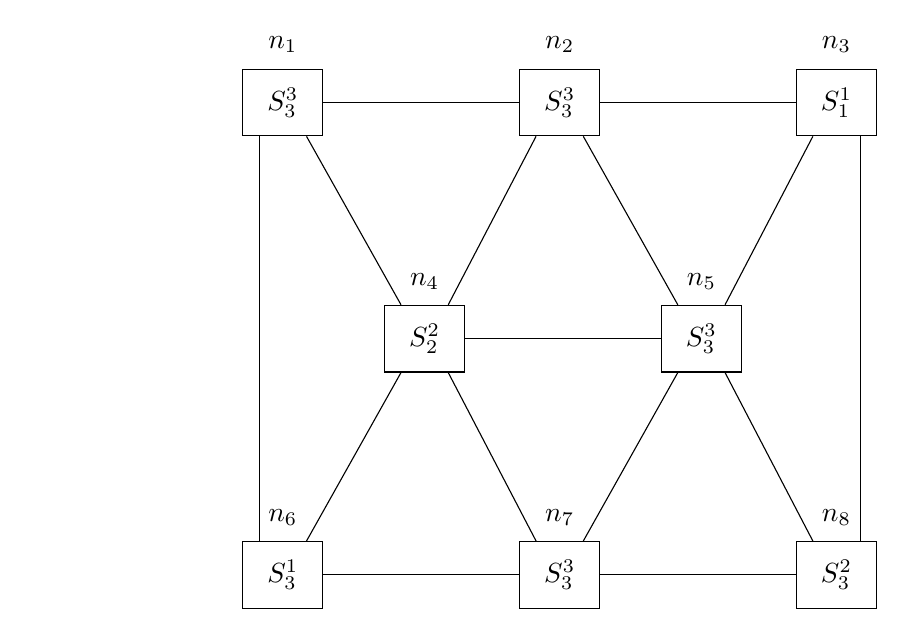
\begin{tikzpicture}

\pgfmathsetmacro{\OTX}{3.0}
\pgfmathsetmacro{\INY}{0.3}
\pgfmathsetmacro{\OTY}{3.0}

\node [] (start) at (0, 0) {};
\node [align=center, minimum height=5ex, minimum width=6ex, draw] (n1) at
($(start.east) + (\OTX, 0)$) {$S_{3}^{3}$};
\node [] at ($(n1.north) + (0, \INY)$) {$n_1$};

\node [align=center, minimum height=5ex, minimum width=6ex, draw] (n2) at
($(n1.east) + (\OTX, 0)$) {$S_{3}^{3}$};
\node [] at ($(n2.north) + (0, \INY)$) {$n_2$};

\node [align=center, minimum height=5ex, minimum width=6ex, draw] (n3) at
($(n2.east) + (\OTX, 0)$) {$S_{1}^{1}$};
\node [] at ($(n3.north) + (0, \INY)$) {$n_3$};

\node [align=center, minimum height=5ex, minimum width=6ex, draw] (n4) at
($(n1) + (\OTX/2+\INY, -\OTY)$) {$S_{2}^{2}$};
\node [] at ($(n4.north) + (0, \INY)$) {$n_4$};

\node [align=center, minimum height=5ex, minimum width=6ex, draw] (n5) at
($(n2) + (\OTX/2+\INY, -\OTY)$) {$S_{3}^{3}$};
\node [] at ($(n5.north) + (0, \INY)$) {$n_5$};

\node [align=center, minimum height=5ex, minimum width=6ex, draw] (n6) at
($(n1) + (0, -\OTY*2)$) {$S_{3}^{1}$};
\node [] at ($(n6.north) + (0, \INY)$) {$n_6$};

\node [align=center, minimum height=5ex, minimum width=6ex, draw] (n7) at
($(n6.east) + (\OTX, 0)$) {$S_{3}^{3}$};
\node [] at ($(n7.north) + (0, \INY)$) {$n_7$};

\node [align=center, minimum height=5ex, minimum width=6ex, draw] (n8) at
($(n7.east) + (\OTX, 0)$) {$S_{3}^{2}$};
\node [] at ($(n8.north) + (0, \INY)$) {$n_8$};

\draw [-] (n1.east) -- (n2.west);
\draw [-] (n2.east) -- (n3.west);
\draw [-] (n4.east) -- (n5.west);
\draw [-] (n6.east) -- (n7.west);
\draw [-] (n7.east) -- (n8.west);

\draw [-] ($(n1.south) + (-\INY, 0)$) -- ($(n6.north) + (-\INY, 0)$);
\draw [-] ($(n3.south) + (\INY, 0)$) -- ($(n8.north) + (\INY, 0)$);

\draw [-] ($(n1.south) + (\INY, 0)$) -- ($(n4.north) + (-\INY, 0)$);
\draw [-] ($(n6.north) + (\INY, 0)$) -- ($(n4.south) + (-\INY, 0)$);
\draw [-] ($(n2.south) + (-\INY, 0)$) -- ($(n4.north) + (\INY, 0)$);
\draw [-] ($(n7.north) + (-\INY, 0)$) -- ($(n4.south) + (\INY, 0)$);

\draw [-] ($(n2.south) + (\INY, 0)$) -- ($(n5.north) + (-\INY, 0)$);
\draw [-] ($(n7.north) + (\INY, 0)$) -- ($(n5.south) + (-\INY, 0)$);
\draw [-] ($(n3.south) + (-\INY, 0)$) -- ($(n5.north) + (\INY, 0)$);
\draw [-] ($(n8.north) + (-\INY, 0)$) -- ($(n5.south) + (\INY, 0)$);

\end{tikzpicture}

对于区块链系统中的任意一个节点$n_i$,在某一时刻$t$,节点状态为$S_{m}^{j}$,即节点中包含协议集合$\{p_1,p_2,..,p_j,..,p_m\}$,且当前运行的协议为$p_j$。
显然,对于不同节点,节点状态存在差异(节点中包含的协议集合不同或当前运行的协议不同)。
在默认条件下(未被外部请求调用),对于已经达成共识的节点的状态总是为$S_{m}^{m}$($p_m$为最新协议),即包含了完整的协议集合,运行着最新的协议。

以上述模型为例,区块链系统中节点$n_1$、$n_2$、$n_5$、$n_7$处于默认状态下($S_{3}^{3}$,包含协议集合$\{p_1,p_2,p_3\}$,当前运行协议$p_3$),其余节点的状态与默认状态不一致。
导致节点运行在非默认状态下的原因有:
1)节点正在进行数据同步,执行历史协议版本、验证交易,如$n_3$、$n_4$;
2)节点被外部请求调用,正在执行外部指定的协议,如$n_6$、$n_8$。

当区块链系统中发布协议($p_4$)更新时,协议会被广播到全网,且只有达成最新共识的节点会接收到$p_4$。
$p_4$会更新到节点包含的协议集合,且更新节点当前运行的协议,即节点状态更新为$S_{4}^{4}$。

\subsection{协议发布}
基于对区块链系统中协议的狭义、广义定义,协议以区块链系统作为底层库,实现某种需求或功能;
更进一步,协议可以实现底层库的功能,成为提供服务的一方。
总之,协议实质上是一份源代码。
另一方面,协议需要在区块链系统中发布,达成共识,并广播到全网,而区块链系统中交易的性质恰好满足协议发布、共识、全网广播的性质,可以考虑协议同交易一起打包。

\subsection{版本管理}
文章之前已经阐述在区块链系统升级协议时,会有不同版本的协议产生,这就导致需要对协议版本进行管理。
协议的版本管理主要分为两部分:处理接收的更新协议,和返回对于某个协议的请求。
对于前者,在接收到新协议(上文已经提到可通过交易发布协议,即接收交易)时,能够解析交易、提取协议;
更进一步,为了维护不同版本的协议,需要保存协议。
对于后者,在接收到请求时,能够快速检索满足条件的协议。

\subsection{执行引擎}
一般而言,外部请求某个协议后,紧接着是对该协议的执行。
对于系统而言,执行效率是需要考虑的问题。
上文中已经提到协议的本质是源代码,执行源代码的前提条件是源代码可被机器识别,且相关依赖已准备就绪。
显然,从交易中解析提取的协议实体并不满足条件:
协议源代码是高级语言,机器无法直接识别执行,需要编译、链接、解释;
其相关依赖也面临着同样的问题。
然而,在每一次请求到来时,再对协议编译、链接、解释又显得不切实际,这严重影响了系统的执行效率,对性能造成灾难行的后果。

解决方案之一是上文提及的即时编译技术。
外部请求返回的协议实体是已被翻译的语言,即时编译引擎在执行时只需要去查找相关符号是否在库的符号表中,无需编译、链接过程,可动态地解释。
以上方案要求解析交易、获取协议实体时额外再做一件事:
将协议转化为可被即时编译引擎直接执行的语言。
如此,便保证了在外部请求下,返回的协议实体可被直接执行。

% !TEX root = main.tex
\section{Overview}

Overview section.

% !TEX root = main.tex

\section{系统实现}

本章详细说明中间表示模块和即时编译引擎的实现细节,包括其中的设计思想以及算法的具体实现。
对于系统中其它模块的具体实现,并不是文章的重点,就不再详细说明。

\subsection{中间表示管理模块}

中间表示管理模块接收协议表示集合,插入并发执行代码到协议表示集合中。
其中实施插入并发执行代码的过程具体分为以下几个阶段:
\begin{itemize}
  \item 初始化阶段。
  通过协议表示集合的$.data$字段获取协议表示集合中的共享变量。
  对每一个共享变量都维护一个数据结构,包括共享变量的版本号以及写锁,其中版本号初始化为$0$,写锁初始化为打开。
  对共享变量所在的协议表示,维护一对读写集,以日志事件的形式记录对共享变量的读写操作,读集和写集初始化都为空。
  维护一个全局版本的时钟,对每一次执行操作,都有一个当前执行的读版本,当前执行的读版本初始化为全局版本时钟。

  \item 执行阶段。
  对于读集,会将读取共享变量地址加入到读集的条目中;
  对于写集,会将写入共享变量地址和值加入到写集中。
  读操作会先访问写集,若写集中存在要访问的共享变量地址,读操作直接将写集中对应共享变量地址对应地取出,否则读操作直接访问共享变量;
  除此之外,需要检查该共享变量地址版本是否小于等于当前执行版本,以及共享变量是否上锁,若不满足条件则说明共享变量正在被修改或已经被修改,需要立即中止执行;
  写操作会直接将共享变量地址及与之对应的数值写入写集,并检查共享变量版本号及锁,不满足立即中止执行。

  \item 提交阶段。
  对全局版本锁进行自增操作,并设置当前执行的写版本为自增后的全局版本锁。
  对读集提交,检查共享内存版本号及是否上锁。
  对写集提交,对每个共享变量上锁,将写集的日志更新到变量,并将共享变量版本更新为当前执行的写版本,解锁共享变量。

\end{itemize}

\subsection{即时编译引擎}

% !TEX root = main.tex

\section{系统评估}


%% !TEX root = main.tex

\section{总结}


\newpage
\bibliography{reference}

\end{document}
